\let\negmedspace\undefined
\let\negthickspace\undefined
\documentclass[journal]{IEEEtran}
\usepackage[a5paper, margin=10mm, onecolumn]{geometry}
%\usepackage{lmodern} % Ensure lmodern is loaded for pdflatex
\usepackage{tfrupee} % Include tfrupee package

\setlength{\headheight}{1cm} % Set the height of the header box
\setlength{\headsep}{0mm}     % Set the distance between the header box and the top of the text

\usepackage{gvv-book}
\usepackage{gvv}
\usepackage{cite}
\usepackage{amsmath,amssymb,amsfonts,amsthm}
\usepackage{algorithmic}
\usepackage{graphicx}
\usepackage{textcomp}
\usepackage{xcolor}
\usepackage{txfonts}
\usepackage{listings}
\usepackage{enumitem}
\usepackage{mathtools}
\usepackage{gensymb}
\usepackage{comment}
\usepackage[breaklinks=true]{hyperref}
\usepackage{tkz-euclide} 
\usepackage{listings}
% \usepackage{gvv}                                        
\def\inputGnumericTable{}                                 
\usepackage[latin1]{inputenc}                                
\usepackage{color}                                            
\usepackage{array}                                            
\usepackage{longtable}                                       
\usepackage{calc}                                             
\usepackage{multirow}                                         
\usepackage{hhline}                                           
\usepackage{ifthen}                                           
\usepackage{lscape}
\begin{document}

\bibliographystyle{IEEEtran}
\vspace{3cm}

\title{9.5.7}
\author{EE24BTECH11011-B.PRANAY KUMAR
}
 \maketitle
% \newpage
% \bigskip
{\let\newpage\relax\maketitle}

\renewcommand{\thefigure}{\theenumi}
\renewcommand{\thetable}{\theenumi}
\setlength{\intextsep}{10pt} % Space between text and floats


\numberwithin{equation}{enumi}
\numberwithin{figure}{enumi}
\renewcommand{\thetable}{\theenumi}



\textbf{Question}:\\
Find the solution of the pair of equations 
\begin{align}
    \frac{3}{x}+\frac{8}{y}= -1 , \frac{1}{x} - \frac{2}{y}= 2 , x,y \neq 0
\end{align}

\solution
\begin{table}[h!]    
  \centering
  \begin{tabular}[12pt]{ |c| |c| }
    \hline
    \textbf{Property} & \textbf{Value} \\ 
    \hline
    Triangle Name & $ \triangle PQR $ \\ 
    \hline
    Side $ QR $ & 3 cm \\ 
    \hline
    Condition on Sides & $ QP - PR = 6 $ cm \\ 
    \hline
    Angle $ \angle PQR $ &  $45^\circ $ \\ 
    \hline
\end{tabular}

  \caption{Variables Used}
  \label{table 9.5.7}
\end{table}\\
To solve using matrices, let's rewrite the equations in a simpler form by letting:


$a = \frac{1}{x}$, $ b = \frac{1}{y}$


The equations become:
\begin{align}
3a + 8b = -1\\
a - 2b = 2
\end{align}

We can represent the system in matrix form as:

\begin{align}
\myvec {3 & 8 \\ 1 & -2 } \myvec{a \\ b } = \myvec{-1 \\ 2 }
\end{align}

The system can be represented in augmented matrix form as:
\begin{align}
\myvec{3 & 8 & -1 \\
1 & -2 & 2}
\xleftrightarrow[]{R_2 \rightarrow {3R_2-R_1}}
\myvec{3 & 8 & -1\\
0 & -14 & 7}
\end{align}
\begin{align}
   \myvec{3 & 8 & -1\\
0 & -14 & 7}
\xleftrightarrow[]{R_2 \rightarrow {\frac{R_2}{-7}}}
\myvec{3 & 8 & -1\\
0 & 2 & -1}
\xleftrightarrow[]{R_1 \rightarrow {R_1-4R_2}}
\myvec{3 & 0 & 3\\
0 & 2 & -1}
\end{align}
\begin{align}
\myvec{1 & 0 & 1\\
0 & 1 & \frac{-1}{2}}
\end{align}
Therefore ;
\begin{align}
    a = 1 , b = \frac{-1}{2}
\end{align}
As $a = \frac{1}{x}$, $ b = \frac{1}{y}$ we get :
\begin{align}
    x = 1 , y = -2
\end{align}
\begin{figure}[h!]
   \centering
   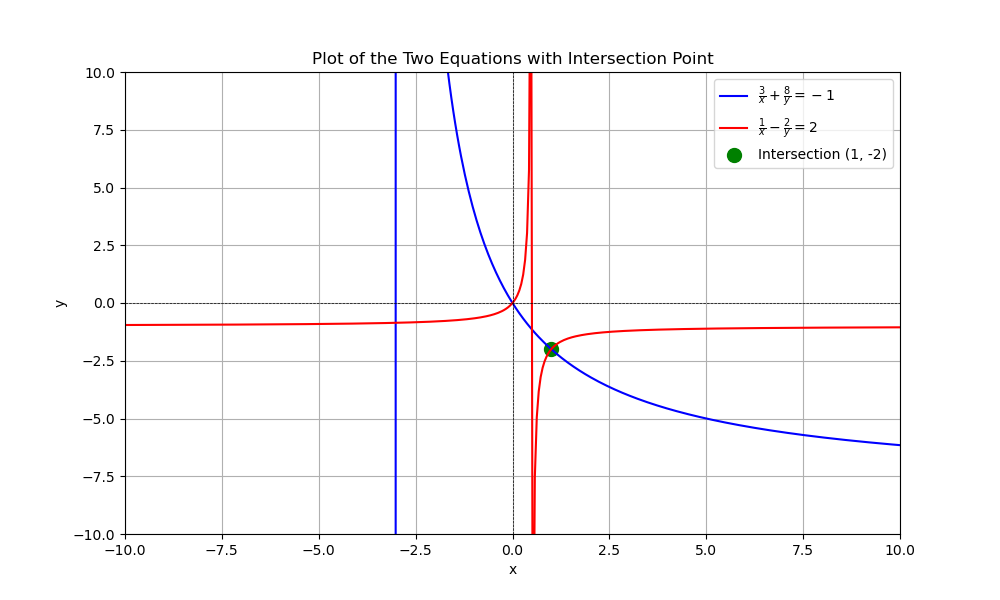
\includegraphics[width=0.7\linewidth]{figs/Q3.png}
   \caption{System of equations}
\end{figure}

\end{document}


